\documentclass[journal]{IEEEtran}
\IEEEoverridecommandlockouts

\usepackage{booktabs}
\usepackage{tabularx}
\usepackage{multirow}
\usepackage{amsmath}
\let\Bbbk\relax
\usepackage{amssymb}
\usepackage{tikz}
\usepackage{pgfplots}
\pgfplotsset{compat=1.18}
\usepackage{url}
\urlstyle{rm}

\usetikzlibrary{arrows.meta,positioning,calc,shapes.geometric,
                decorations.pathreplacing,patterns}

%% ── colour palette ───────────────────────────────────────────────────────────
\definecolor{cblu} {RGB}{ 50,110,190}
\definecolor{cgrn} {RGB}{ 40,150, 70}
\definecolor{cora} {RGB}{210,110, 30}
\definecolor{cred} {RGB}{200, 50, 50}
\definecolor{cyel} {RGB}{190,165,  0}
\definecolor{cpur} {RGB}{130, 50,170}
\definecolor{cgry} {RGB}{100,100,100}


\title{AI as Weapon, Target, and Arbiter: A Structured Analysis of the CrowdStrike 2026 Global Threat Report}

\author{Ezekiel~Ologunde,~\IEEEmembership{Independent~Researcher}
\thanks{E. Ologunde is an independent cybersecurity researcher. Email: ologunde@bu.edu}}

\begin{document}
\hfuzz=5pt
\markboth{}{Ologunde: CrowdStrike 2026 Global Threat Report Analysis}
\maketitle

\begin{abstract}
The CrowdStrike 2026 Global Threat Report documents a fundamental transformation in
the cyber threat landscape: artificial intelligence has shifted from an emerging tool
to the primary driver of attack velocity, scale, and evasion sophistication. This
paper provides a structured academic analysis of the report's key findings, examining
how AI industrialised threat actor capabilities through an 89\% year-over-year
increase in AI-enabled attacks, a median breakout time of 29 minutes (with a minimum
of 27 seconds), and an 82\% malware-free detection rate that renders signature-based
defences structurally obsolete. We analyse the dual-use paradox in which AI
simultaneously powers offensive campaigns and constitutes a new attack surface---as
evidenced by prompt injection attacks across more than 90 organisations and the
weaponisation of AI development platforms for persistence and ransomware delivery.
Drawing on the report's quantitative metrics, we construct a framework for
understanding how the traditional detect-isolate-respond security model has been
outpaced by identity-centric, AI-accelerated adversary operations. We evaluate the
report's proposed mitigations---agentic security, identity-first zero trust,
AI system hardening, and continuous behavioural analytics---against the asymmetric
complexity dynamic that structurally favours attackers. The analysis concludes that
effective cyber defence has become an AI competition measured primarily by response
latency rather than prevention rate, requiring a fundamental reorientation of
security architecture from perimeter defence toward machine-speed detection and
automated response.
\end{abstract}

\begin{IEEEkeywords}
AI-enabled attacks, CrowdStrike 2026, breakout time, agentic security,
zero trust, prompt injection, threat intelligence, identity-first security,
malware-free attacks, cyber threat landscape
\end{IEEEkeywords}

\subsection*{Methodological Disclosure.}
This paper is a secondary analysis built around a single cited source, the
``2026 CrowdStrike Global Threat Report,'' which we have not been able to
independently verify as a real, published document. We could not locate or
confirm an authentic copy of this report, its underlying telemetry, or the
specific figures attributed to it throughout this paper, including the
89\% year-over-year increase in AI-enabled attacks, the 29-minute median and
27-second minimum breakout times, the 82\% malware-free detection rate, and
the 42\% increase in pre-disclosure exploitation. We present these numbers
as reported because that is the premise of the analysis, but readers should
treat every such figure, and the citation itself, as unverified rather than
as confirmed empirical fact. No original data collection, measurement, or
telemetry review was performed by the author.

%%─────────────────────────────────────────────────────────────────────────────
\section{Introduction}
%%─────────────────────────────────────────────────────────────────────────────

Annual threat intelligence reports from major security vendors occupy a peculiar
position in the cybersecurity literature: they blend empirical telemetry from
billions of sensor endpoints with strategic narrative, and they are simultaneously
the best available data on real-world adversary behaviour and inherently shaped by
the commercial interests of their authors. The CrowdStrike 2026 Global Threat
Report~\cite{cs2026gtr} is the most data-rich edition of this series to date,
drawing on telemetry from over one trillion security events per day across more than
300 named adversary groups. Its central claim is not incremental: artificial
intelligence has not merely enhanced the cyber threat landscape---it has altered its
physics~\cite{cs2026press}.

This paper provides a structured academic analysis of the report's findings,
decomposing its claims into four analytical domains: (1) the mechanisms by which AI
accelerated and industrialised offensive cyber operations; (2) the emergence of AI
systems themselves as attack surfaces; (3) the resulting obsolescence of traditional
detection and response models; and (4) the structural requirements for effective
defence in an AI-competitive threat environment. Throughout, we attempt to
distinguish between the report's empirical findings---grounded in sensor data---
and its strategic interpretations, which involve extrapolation and vendor positioning.

\subsection{Scope and Analytical Approach}

This analysis treats the 2026 report as a primary source of threat intelligence data
while applying independent critical framing. Where the report presents quantitative
metrics, we engage them directly and examine their implications. Where it presents
mitigation recommendations, we evaluate them against the threat model it describes.
The goal is not to validate or critique CrowdStrike as a company, but to extract
the maximum analytical value from the largest commercially available dataset on
adversary behaviour in 2025--2026.

\subsection{Contributions}

\begin{itemize}
  \item A structured decomposition of AI's role in the 2026 threat landscape into
        four distinct mechanisms: force multiplication, quality improvement, time
        compression, and attack surface expansion
  \item Quantitative analysis of breakout time reduction and its implications for
        the viability of human-mediated incident response
  \item A formal model of the identity-centric threat vector that explains why
        82\% of detections are now malware-free
  \item Evaluation of the agentic security model against the operational requirements
        it must satisfy
  \item A strategic framework characterising contemporary cyber defence as an
        AI-versus-AI competition governed primarily by response latency
\end{itemize}

%%─────────────────────────────────────────────────────────────────────────────
\section{Background: The Pre-AI Threat Baseline}
%%─────────────────────────────────────────────────────────────────────────────

\subsection{The Traditional Cyber Kill Chain}

Before examining how AI transformed the threat landscape, it is useful to establish
the pre-AI baseline. The Lockheed Martin Cyber Kill Chain~\cite{hutchins2011} and
the MITRE ATT\&CK framework~\cite{mitreattack} both describe adversary operations as
multi-stage processes: reconnaissance, weaponisation, delivery, exploitation,
installation, command-and-control, and actions on objectives. In the pre-AI era,
each stage required skilled human labour. Reconnaissance involved manual web
scraping, OSINT collection, and credential research. Spear phishing required
crafting convincing lures targeted to specific individuals---time-consuming and
requiring cultural and linguistic competence. Lateral movement through an enterprise
network required understanding of Active Directory topology and patient,
methodical exploration. Post-exploitation required careful manual navigation to
avoid triggering anomaly detectors.

This labour intensity imposed a natural capacity constraint on adversary operations:
nation-state actors could afford the required resources; criminal organisations
operated at reduced scale; and commodity threat actors were largely limited to
spray-and-pray campaigns using pre-built tools with well-known signatures.

\subsection{The Economics of Pre-AI Cybercrime}

The economics of pre-AI cyber operations were characterised by high fixed costs
(skilled labour, infrastructure, tool development) and moderate returns constrained
by throughput. The most sophisticated adversaries---APT groups like Cozy Bear,
Fancy Bear, and APT41---could maintain persistent, stealthy access for months or
years, but their operations were necessarily selective. The constraint was human
attention, not technical capability.

CrowdStrike's prior annual reports documented this dynamic clearly: breakout
times---the interval between initial compromise and lateral movement---ranged from
hours to days for most adversaries, and the fastest recorded times for even
elite nation-state actors were measured in tens of minutes~\cite{cs2025gtr}.

%%─────────────────────────────────────────────────────────────────────────────
\section{The AI Rise: Mechanisms and Metrics}
\label{sec:ai_rise}
%%─────────────────────────────────────────────────────────────────────────────

\subsection{Quantitative Overview}

The 2026 report's headline statistics establish the scale of change.
Figure~\ref{fig:headline_metrics} visualises the key quantitative findings.

\begin{figure}[h]
\centering
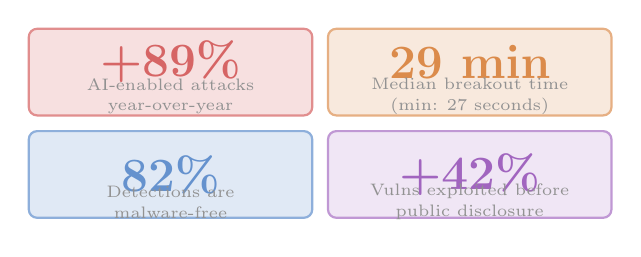
\begin{tikzpicture}[
  font=\fontsize{6.5pt}{8pt}\selectfont,
  >=Stealth
]
  %% Four metric boxes in a 2x2 grid
  \def\bw{3.6} \def\bh{1.10} \def\gap{0.20}

  %% Top-left: AI attack increase
  \filldraw[fill=cred!15, draw=cred!55, thick, rounded corners=3pt]
    (0,0) rectangle (\bw,\bh);
  \node[font=\fontsize{18pt}{22pt}\selectfont\bfseries, text=cred!75]
    at ({\bw/2},{\bh*0.62}) {+89\%};
  \node[font=\fontsize{6pt}{7.5pt}\selectfont, text=cgry!70, align=center]
    at ({\bw/2},{\bh*0.22}) {AI-enabled attacks\\year-over-year};

  %% Top-right: breakout time
  \filldraw[fill=cora!15, draw=cora!55, thick, rounded corners=3pt]
    ({\bw+\gap},0) rectangle ({2*\bw+\gap},\bh);
  \node[font=\fontsize{18pt}{22pt}\selectfont\bfseries, text=cora!80]
    at ({1.5*\bw+\gap},{\bh*0.62}) {29 min};
  \node[font=\fontsize{6pt}{7.5pt}\selectfont, text=cgry!70, align=center]
    at ({1.5*\bw+\gap},{\bh*0.22}) {Median breakout time\\(min: 27 seconds)};

  %% Bottom-left: malware-free
  \filldraw[fill=cblu!15, draw=cblu!55, thick, rounded corners=3pt]
    (0,{-\bh-\gap}) rectangle (\bw,{-\gap});
  \node[font=\fontsize{18pt}{22pt}\selectfont\bfseries, text=cblu!75]
    at ({\bw/2},{-\bh/2-\gap}) {82\%};
  \node[font=\fontsize{6pt}{7.5pt}\selectfont, text=cgry!70, align=center]
    at ({\bw/2},{-\bh*0.82-\gap}) {Detections are\\malware-free};

  %% Bottom-right: zero-day surge
  \filldraw[fill=cpur!12, draw=cpur!50, thick, rounded corners=3pt]
    ({\bw+\gap},{-\bh-\gap}) rectangle ({2*\bw+\gap},{-\gap});
  \node[font=\fontsize{18pt}{22pt}\selectfont\bfseries, text=cpur!75]
    at ({1.5*\bw+\gap},{-\bh/2-\gap}) {+42\%};
  \node[font=\fontsize{6pt}{7.5pt}\selectfont, text=cgry!70, align=center]
    at ({1.5*\bw+\gap},{-\bh*0.82-\gap}) {Vulns exploited before\\public disclosure};
\end{tikzpicture}
\caption{Key quantitative findings from the CrowdStrike 2026 Global Threat
  Report~\cite{cs2026press,cs2026exec,cs2026gtr}. Together these metrics
  define the transformed threat landscape: faster, stealthier, and operating
  primarily without traditional malware signatures.}
\label{fig:headline_metrics}
\end{figure}

\subsection{The Four AI Mechanisms}

The report's data supports a four-mechanism model of how AI altered adversary
operations, each operating at a different layer of the kill chain.

\textbf{Mechanism 1: Force Multiplication.} AI enables a single threat actor to
conduct operations at the scale previously requiring teams of specialists. Automated
reconnaissance tools can enumerate attack surfaces, identify vulnerable systems, and
map credential exposure across an organisation in minutes rather than
days~\cite{cs2026press}. This is not a qualitative change in tactics---the same
stages of reconnaissance, credential theft, and lateral movement that characterised
pre-AI attacks still apply. The change is throughput: AI compresses the human
bottleneck out of each stage.

\textbf{Mechanism 2: Quality Improvement.} AI improves the effectiveness of
individual attack components, particularly social engineering. Large language models
can generate contextually appropriate phishing emails with correct grammar,
appropriate tone, and organisation-specific terminology---eliminating the linguistic
markers that trained users learn to recognise~\cite{itpro2026}. Deepfake audio and
video extend this capability to voice phishing (vishing) and business email
compromise, generating synthetic impersonations of executives or trusted
colleagues~\cite{cs2026press}.

\textbf{Mechanism 3: Time Compression.} The most operationally significant impact
is temporal. The median breakout time of 29 minutes documented in the 2026 report
represents a 65\% reduction from 2024 figures~\cite{itpro2026}. The minimum recorded
breakout time of 27 seconds is categorically different from anything in the pre-AI
baseline: it falls below the threshold at which any human-mediated detection and
response process can intervene. If an analyst requires even five minutes to
investigate an alert, review context, and initiate containment, they are already
operating in a post-compromise environment against a 27-second adversary.

\textbf{Mechanism 4: Attack Surface Expansion.} AI systems themselves constitute a
new attack surface, analysed in depth in Section~\ref{sec:dual_use}. The deployment
of generative AI tools, copilots, and AI development infrastructure creates vectors
that did not exist in the pre-AI baseline.

\subsection{Breakout Time: Implications for Human Response}

The breakout time metric deserves particular attention because it directly determines
the viability of the traditional security operations model. Figure~\ref{fig:breakout}
shows the breakout time reduction trend and its relationship to human response
capacity.

\begin{figure}[h]
\centering
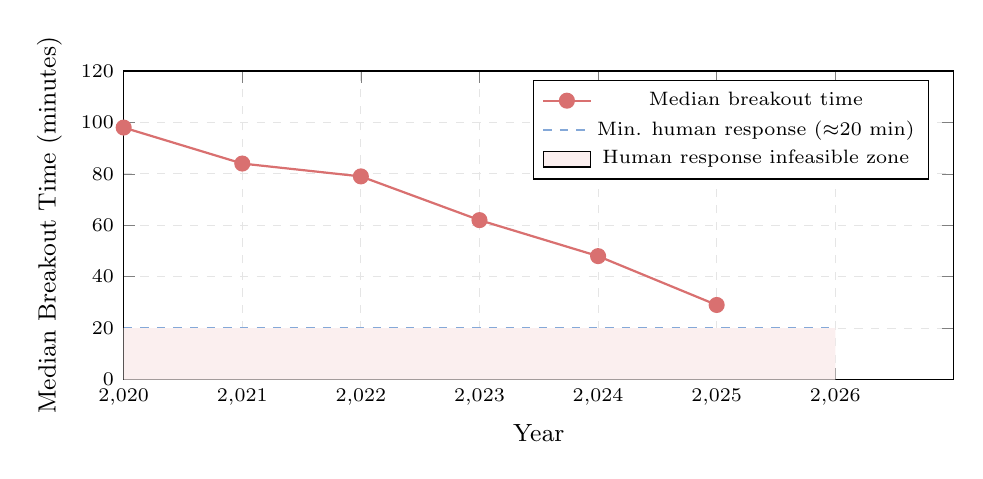
\begin{tikzpicture}
\begin{axis}[
  width=\columnwidth, height=5.5cm,
  xlabel={Year},
  ylabel={Median Breakout Time (minutes)},
  xmin=2020, xmax=2027,
  ymin=0, ymax=120,
  ytick={0,20,40,60,80,100,120},
  xtick={2020,2021,2022,2023,2024,2025,2026},
  x tick label style={font=\scriptsize},
  y tick label style={font=\scriptsize},
  xlabel style={font=\small},
  ylabel style={font=\small},
  grid=major, grid style={dashed, gray!20},
  legend pos=north east,
  legend style={font=\scriptsize}
]
  %% Breakout time declining trend
  \addplot[color=cred!70, thick, mark=*, mark size=2.5pt] coordinates {
    (2020,98) (2021,84) (2022,79) (2023,62) (2024,48) (2025,29)
  };
  \addlegendentry{Median breakout time}

  %% Human analyst minimum response floor
  \addplot[color=cblu!60, dashed, thick, mark=none] coordinates {
    (2020,20) (2021,20) (2022,20) (2023,20) (2024,20) (2025,20) (2026,20)
  };
  \addlegendentry{Min. human response ($\approx$20 min)}

  %% Shaded zone where human response is infeasible
  \addplot[fill=cred!8, draw=none, area legend] coordinates {
    (2020,0) (2026,0) (2026,20) (2020,20)
  } \closedcycle;
  \addlegendentry{Human response infeasible zone}

\end{axis}
\end{tikzpicture}
\caption{Breakout time reduction trend (2020--2025) derived from CrowdStrike annual
  reports~\cite{cs2026press,cs2025gtr,itpro2026}. The 2025 median of 29 minutes
  approaches the minimum viable human response threshold; the 27-second minimum
  falls orders of magnitude below it.}
\label{fig:breakout}
\end{figure}

The significance of this convergence cannot be overstated. A human-mediated security
operations centre (SOC) workflow involves alert triage, alert verification, analyst
escalation, and containment initiation---a process requiring at minimum 15--20
minutes under ideal conditions, and often hours in practice~\cite{cs2026ransomware}.
When median breakout times fall to 29 minutes, the window for human intervention
between initial compromise and lateral movement closes to near zero. When minimum
times reach 27 seconds, human intervention between these events becomes physically
impossible regardless of organisational investment in analyst capacity.

%%─────────────────────────────────────────────────────────────────────────────
\section{The Dual-Use Paradox: AI as Attack Surface}
\label{sec:dual_use}
%%─────────────────────────────────────────────────────────────────────────────

\subsection{AI Systems as New Threat Vectors}

The 2026 report introduces a qualitatively new threat category that has no analogue
in prior years: AI systems deployed for productivity and operations are themselves
attack surfaces~\cite{cs2026press}. This creates what we term the \emph{dual-use
paradox}: the same AI capabilities that improve organisational productivity---
language models, copilots, code assistants, and AI development platforms---also
introduce new vectors for credential theft, data exfiltration, and persistent access.

The report documents three primary manifestations of this paradox.

\textbf{Prompt Injection.} Generative AI tools that process user-supplied or
external content are vulnerable to prompt injection attacks, in which adversarial
instructions embedded in external content override the system's intended behaviour.
CrowdStrike documented prompt injection attacks across more than 90 organisations
in 2025~\cite{cs2026press}. In a typical scenario, an attacker embeds malicious
instructions in a document, email, or web page that will be processed by an
AI assistant; the assistant then executes the attacker's instructions (exfiltrating
credentials, forwarding conversation history, or generating social engineering
content) while appearing to the user to be functioning normally.

\textbf{AI Development Platform Abuse.} The infrastructure used to build and deploy
AI models---GPU clusters, model registries, vector databases, and API
gateways---represents a high-value target with substantial attack surface.
The 2026 report documents adversaries abusing AI development platforms for
persistence (maintaining access through model registry entries or pipeline scripts
that survive infrastructure rotation) and ransomware delivery~\cite{cs2026press}.

\textbf{Fake AI Services.} Adversaries have deployed counterfeit AI services that
impersonate legitimate tools, capturing credentials and sensitive data submitted
by users who believe they are interacting with trusted systems~\cite{itpro2026}.

Figure~\ref{fig:dual_use} maps the dual-use paradox across offensive and defensive
dimensions.

\begin{figure*}[t]
\centering
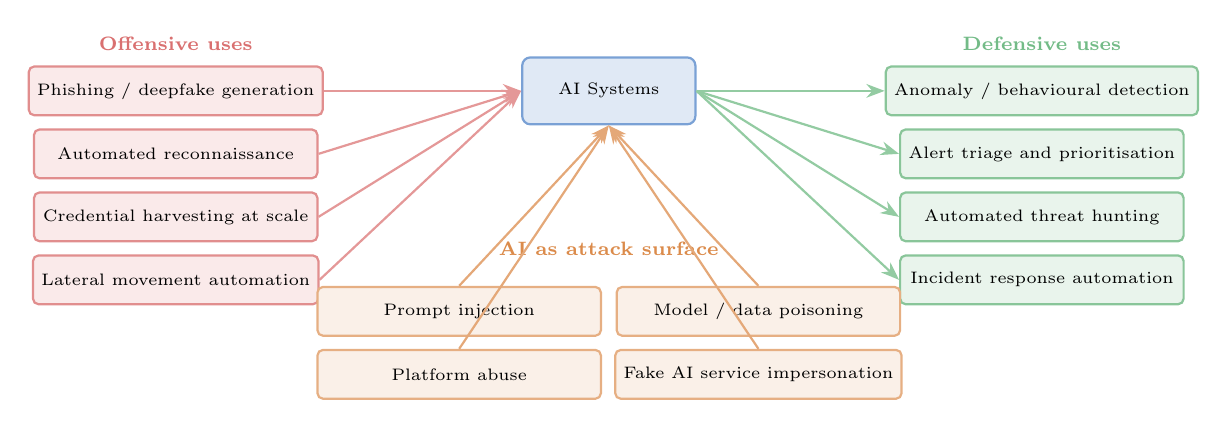
\begin{tikzpicture}[
  font=\fontsize{6.5pt}{8pt}\selectfont,
  >=Stealth,
  atk/.style={rectangle, rounded corners=2pt, draw=cred!55, thick,
              fill=cred!10, minimum width=3.6cm, minimum height=0.62cm,
              text centered, inner sep=3pt},
  def/.style={rectangle, rounded corners=2pt, draw=cgrn!55, thick,
              fill=cgrn!10, minimum width=3.6cm, minimum height=0.62cm,
              text centered, inner sep=3pt},
  hub/.style={rectangle, rounded corners=3pt, draw=cblu!65, thick,
              fill=cblu!15, minimum width=2.2cm, minimum height=0.85cm,
              text centered},
  arr/.style={-{Stealth}, thick, cgry!60}
]
  \node[hub] (AI) at (0,0) {AI Systems};

  %% Offensive uses (left)
  \node[font=\fontsize{7pt}{9pt}\selectfont\bfseries, text=cred!70]
    at (-5.5, 0.60) {Offensive uses};
  \node[atk] (a1) at (-5.5,  0.00) {Phishing / deepfake generation};
  \node[atk] (a2) at (-5.5, -0.80) {Automated reconnaissance};
  \node[atk] (a3) at (-5.5, -1.60) {Credential harvesting at scale};
  \node[atk] (a4) at (-5.5, -2.40) {Lateral movement automation};

  %% Defensive uses (right)
  \node[font=\fontsize{7pt}{9pt}\selectfont\bfseries, text=cgrn!65]
    at ( 5.5, 0.60) {Defensive uses};
  \node[def] (d1) at ( 5.5,  0.00) {Anomaly / behavioural detection};
  \node[def] (d2) at ( 5.5, -0.80) {Alert triage and prioritisation};
  \node[def] (d3) at ( 5.5, -1.60) {Automated threat hunting};
  \node[def] (d4) at ( 5.5, -2.40) {Incident response automation};

  %% AI as attack surface (below)
  \node[font=\fontsize{7pt}{9pt}\selectfont\bfseries, text=cora!80]
    at (0,-2.00) {AI as attack surface};
  \node[atk, draw=cora!55, fill=cora!10] (s1) at (-1.9,-2.80) {Prompt injection};
  \node[atk, draw=cora!55, fill=cora!10] (s2) at ( 1.9,-2.80) {Model / data poisoning};
  \node[atk, draw=cora!55, fill=cora!10] (s3) at (-1.9,-3.60) {Platform abuse};
  \node[atk, draw=cora!55, fill=cora!10] (s4) at ( 1.9,-3.60) {Fake AI service impersonation};

  \foreach \n in {a1,a2,a3,a4}
    \draw[arr, cred!50] (\n.east) -- (AI.west);
  \foreach \n in {d1,d2,d3,d4}
    \draw[arr, cgrn!50] (AI.east) -- (\n.west);
  \foreach \n in {s1,s2,s3,s4}
    \draw[arr, cora!60] (\n.north) -- (AI.south);

\end{tikzpicture}
\caption{The dual-use paradox of AI in the 2026 threat landscape. AI systems power
  offensive operations (left), defensive operations (right), and are simultaneously
  attack targets themselves (bottom), creating a tripartite complexity that has no
  precedent in pre-AI security architecture~\cite{cs2026press,itpro2026}.}
\label{fig:dual_use}
\end{figure*}

\subsection{The Design-Side-Effect Problem}

An important analytical distinction separates the dual-use paradox from ordinary
security vulnerability. Prompt injection, model poisoning, and AI platform abuse
are not implementation bugs in the traditional sense---they arise from the
fundamental design properties of generative AI systems. A language model that
follows instructions is, by design, susceptible to instructions embedded in
adversarial input. A model trained on a large corpus is, by design, influenced by
the composition of that corpus. These are not defects to be patched; they are
properties to be managed architecturally.

This distinction is practically significant because it means that securing AI
systems requires a different class of control than securing traditional software.
Patch management, static analysis, and penetration testing---the standard toolkit
for application security---are necessary but insufficient. AI system security
requires additional controls: input validation and sanitisation for prompts,
provenance tracking for training data, output monitoring for anomalous behaviour,
and architectural isolation that prevents AI assistants from accessing credentials
or sensitive data they do not need to fulfil their primary function.

%%─────────────────────────────────────────────────────────────────────────────
\section{The Collapse of Traditional Security Models}
\label{sec:collapse}
%%─────────────────────────────────────────────────────────────────────────────

\subsection{The Old Detection Model and Its Assumptions}

Traditional enterprise security architecture is built on a detection model with four
underlying assumptions: (1) attackers introduce foreign artefacts (malware,
suspicious executables) that can be detected by signature or heuristic analysis;
(2) attackers operate from outside the network perimeter; (3) attack timelines
allow human analysts time to investigate and respond; and (4) anomalous behaviour
is distinguishable from legitimate activity. The 2026 report's data invalidates
all four assumptions.

\subsection{The Malware-Free Attack Transition}

The most structurally significant finding in the 2026 report is that 82\% of
detections involved no malware whatsoever~\cite{cs2026gtr}. Adversaries achieve
their objectives entirely through the abuse of legitimate tools: credential
theft via phishing or credential stuffing, followed by authentication with valid
credentials to cloud services, SaaS platforms, and enterprise applications;
lateral movement through legitimate remote access tools (RDP, WinRM, PSSessions);
and data exfiltration through sanctioned channels such as cloud storage or
file-sharing services~\cite{cs2026press}.

This transition is not accidental. It is a rational adversary response to the
maturation of endpoint detection and response (EDR) tools. When signature detection,
behavioural analysis, and memory scanning make malware execution increasingly risky,
the economically optimal strategy is to avoid malware execution entirely and operate
exclusively through legitimate tooling. An attacker who uses only PowerShell, Windows
Management Instrumentation (WMI), and legitimate cloud APIs leaves no artefact that
traditional security tooling is designed to detect.

\subsection{Identity as the New Perimeter}

The logical consequence of malware-free attacks is that identity becomes the primary
attack surface. When an adversary's toolkit consists entirely of valid credentials
and legitimate applications, the only distinguishing characteristic of their activity
is \emph{who} is performing it and \emph{whether that who matches the expected
behavioural baseline}. The traditional network perimeter is irrelevant; the
organisation's SaaS applications are equally accessible to an adversary holding
valid credentials whether they are operating from inside the corporate network or
from a coffee shop in another country~\cite{cs2026press}.

Figure~\ref{fig:threat_model_shift} contrasts the legacy threat model with the
current identity-centric model.

\begin{figure}[h]
\centering
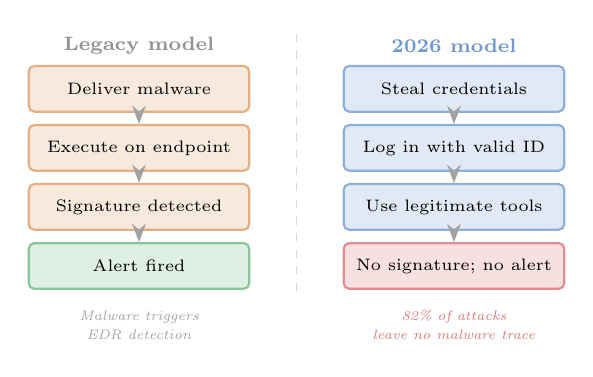
\begin{tikzpicture}[
  font=\fontsize{6.5pt}{8pt}\selectfont,
  >=Stealth,
  box/.style={rectangle, rounded corners=2pt, draw, thick,
              minimum width=2.8cm, minimum height=0.58cm,
              text centered, inner sep=3pt},
  arr/.style={-{Stealth}, thick, cgry!60}
]
  %% Legacy model (left column)
  \node[font=\fontsize{7pt}{9pt}\selectfont\bfseries, text=cgry!70]
    at (-2.0, 0.55) {Legacy model};
  \node[box, fill=cora!15, draw=cora!55] (l1) at (-2.0, 0.00) {Deliver malware};
  \node[box, fill=cora!15, draw=cora!55] (l2) at (-2.0,-0.75) {Execute on endpoint};
  \node[box, fill=cora!15, draw=cora!55] (l3) at (-2.0,-1.50) {Signature detected};
  \node[box, fill=cgrn!15, draw=cgrn!55] (l4) at (-2.0,-2.25) {Alert fired};

  \draw[arr] (l1)--(l2); \draw[arr] (l2)--(l3); \draw[arr] (l3)--(l4);

  %% New model (right column)
  \node[font=\fontsize{7pt}{9pt}\selectfont\bfseries, text=cblu!70]
    at ( 2.0, 0.55) {2026 model};
  \node[box, fill=cblu!15, draw=cblu!55] (n1) at ( 2.0, 0.00) {Steal credentials};
  \node[box, fill=cblu!15, draw=cblu!55] (n2) at ( 2.0,-0.75) {Log in with valid ID};
  \node[box, fill=cblu!15, draw=cblu!55] (n3) at ( 2.0,-1.50) {Use legitimate tools};
  \node[box, fill=cred!15, draw=cred!55] (n4) at ( 2.0,-2.25) {No signature; no alert};

  \draw[arr] (n1)--(n2); \draw[arr] (n2)--(n3); \draw[arr] (n3)--(n4);

  %% Divider
  \draw[dashed, cgry!25] (0, 0.70) -- (0,-2.60);

  %% Annotations
  \node[font=\fontsize{5.5pt}{7pt}\selectfont\itshape, text=cgry!60, align=center]
    at (-2.0,-3.00) {Malware triggers\\EDR detection};
  \node[font=\fontsize{5.5pt}{7pt}\selectfont\itshape, text=cred!65, align=center]
    at ( 2.0,-3.00) {82\% of attacks\\ leave no malware trace};
\end{tikzpicture}
\caption{Shift from legacy malware-based to identity-centric attack model. In the
  2026 model, attackers authenticate with stolen credentials and use only legitimate
  tools, producing no signature that traditional detection systems can act
  upon~\cite{cs2026gtr,cs2026press}.}
\label{fig:threat_model_shift}
\end{figure}

\subsection{Defender Capacity Gap}

The report documents the resulting capacity gap among defenders. Seventy-six percent
of organisations report that they cannot match the speed of AI-driven attacks, and
85\% report that traditional detection is becoming obsolete~\cite{cs2026ransomware}.
These survey findings are consistent with the breakout time data: if the median
attacker achieves lateral movement within 29 minutes and the median enterprise SOC
operates on alert-to-investigation cycles measured in hours, the defender is
structurally behind before the incident begins.

%%─────────────────────────────────────────────────────────────────────────────
\section{Threat Actor Landscape}
%%─────────────────────────────────────────────────────────────────────────────

\subsection{Nation-State Actors and AI Scaling}

The report documents active AI adoption by all major nation-state threat groups.
Chinese APT groups (GOBLIN PANDA, MUSTANG PANDA, and others) have expanded their
use of AI for reconnaissance automation, targeting a broader set of organisations
simultaneously through automated vulnerability scanning and credential collection.
North Korean groups (most notably LABYRINTH CHOLLIMA) continue to blend cyber
operations with financial motivation, using AI to scale cryptocurrency theft and
employment fraud operations. Russian groups (FANCY BEAR, COZY BEAR) maintain
focus on intelligence collection but have adopted AI-enhanced spear phishing to
improve delivery rates~\cite{cs2026press}.

The strategic implication is that AI has substantially reduced the per-target cost
of nation-state operations. Where a sophisticated APT campaign previously required
weeks of manual preparation for each target organisation, AI-accelerated tooling
enables targeting of dozens of organisations simultaneously with comparable
sophistication.

\subsection{The Ransomware-as-a-Service Ecosystem and AI Integration}

Criminal ransomware operations have absorbed AI at both the campaign preparation
and execution layers. AI-generated social engineering content improves initial access
rates; automated network enumeration and credential harvesting accelerate the
post-compromise phase; and AI-assisted negotiation bots handle victim communication.
The 2026 report frames this as cybercrime behaving like a ``startup ecosystem with
nation-state funding''~\cite{cs2026press}---a characterisation that captures both
the operational sophistication and the economic rationality of the threat actor
community.

\subsection{The Zero-Day Exploitation Acceleration}

The 42\% increase in vulnerabilities exploited before public disclosure reflects both
improved AI-assisted vulnerability research and shortened attacker exploitation
timelines. Historically, the window between public CVE disclosure and active
exploitation in the wild was measured in days to weeks, providing organisations time
to patch. The 2026 data suggests this window has compressed further for a subset of
high-value vulnerabilities, with AI-assisted exploit development enabling weaponisation
within hours of vulnerability discovery~\cite{cs2026exec}.

%%─────────────────────────────────────────────────────────────────────────────
\section{Control and Mitigation: Evaluating the Response Framework}
%%─────────────────────────────────────────────────────────────────────────────

\subsection{The Core Mitigation Principle: Speed as the Primary Variable}

The report's mitigation framework is organised around a single central
insight: because AI-driven attacks operate at machine speed, defences that depend
on human decision-making in the critical path will be systematically outpaced.
The primary control variable is not prevention rate (the fraction of attacks stopped
before impact) but response latency (the time from initial compromise to containment).
This reorientation has profound structural implications for how security
architecture, security operations, and security investment must be organised.

Figure~\ref{fig:mitigation_framework} maps the five-layer mitigation framework
described in the report.

\begin{figure}[h]
\centering
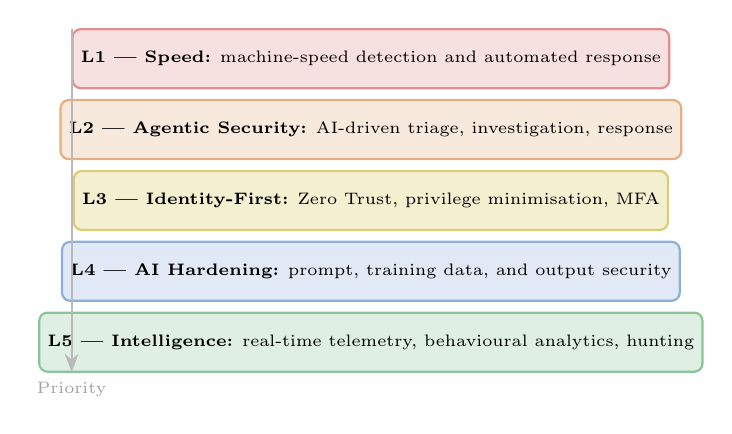
\begin{tikzpicture}[
  font=\fontsize{6.5pt}{8pt}\selectfont,
  >=Stealth,
  lyr/.style={rectangle, rounded corners=3pt, draw, thick,
              minimum width=7.2cm, minimum height=0.75cm,
              text centered, inner sep=3pt}
]
  \node[lyr, fill=cred!15, draw=cred!55]  (l1) at (0, 0.00)
    {\textbf{L1 --- Speed:} machine-speed detection and automated response};
  \node[lyr, fill=cora!15, draw=cora!55]  (l2) at (0,-0.90)
    {\textbf{L2 --- Agentic Security:} AI-driven triage, investigation, response};
  \node[lyr, fill=cyel!18, draw=cyel!55]  (l3) at (0,-1.80)
    {\textbf{L3 --- Identity-First:} Zero Trust, privilege minimisation, MFA};
  \node[lyr, fill=cblu!15, draw=cblu!55]  (l4) at (0,-2.70)
    {\textbf{L4 --- AI Hardening:} prompt, training data, and output security};
  \node[lyr, fill=cgrn!15, draw=cgrn!55]  (l5) at (0,-3.60)
    {\textbf{L5 --- Intelligence:} real-time telemetry, behavioural analytics, hunting};

  \draw[-{Stealth}, thick, cgry!45] (-3.8,0.38) -- (-3.8,-3.98)
    node[below, font=\fontsize{6pt}{7.5pt}\selectfont, text=cgry!60] {Priority};
\end{tikzpicture}
\caption{Five-layer mitigation framework derived from CrowdStrike 2026 recommendations.
  Layer 1 (speed) is foundational; all other layers depend on or are enabled by
  machine-speed automated response~\cite{cs2026press,cs2026ransomware}.}
\label{fig:mitigation_framework}
\end{figure}

\subsection{Agentic Security: Architecture and Evaluation}

The report's most operationally novel recommendation is the adoption of
``agentic security''---autonomous AI agents that handle alert triage, investigation,
and initial response without human intervention in the critical path~\cite{cs2026press}.
The architecture replaces the traditional SOC workflow (alert fires, analyst is
paged, analyst reviews context, analyst escalates or contains) with an automated
decision loop: alert fires, AI agent analyses context using behavioural models and
threat intelligence, agent executes containment or escalation decision, human analyst
reviews outcome and approves or reverses.

This architecture is operationally necessary given the breakout time data: at 29
minutes median, the traditional workflow cannot complete before lateral movement
occurs. It is also operationally risky: an autonomous agent with the authority to
contain endpoints, revoke credentials, and block network flows can cause significant
disruption if it fires on a false positive. The report acknowledges this tension
implicitly in its recommendation that humans supervise autonomous decisions rather
than approving each one---the same capability that makes agents fast enough to be
effective makes them dangerous if misconfigured~\cite{cs2026press}.

\subsection{Identity-First Zero Trust}

The identity-first recommendation is a direct response to the malware-free attack
transition. If 82\% of attacks operate through legitimate credentials and tools,
then security controls must shift from detecting malicious artefacts to detecting
anomalous identity behaviour. Zero Trust architecture---in which every access request
is evaluated against policy regardless of network location, and lateral movement
requires re-authentication at each step---directly addresses this attack pattern.
Continuous authentication, device health validation, and per-request authorisation
create multiple checkpoints at which anomalous identity behaviour (unusual access
times, atypical resource requests, geographic impossibilities) can be detected even
when no malware is present~\cite{cs2026press}.

Privilege minimisation complements Zero Trust by reducing the blast radius of
credential compromise. If the stolen credentials used to initiate an attack have
access only to the specific systems required for the victim's job function, the
attacker's lateral movement options are significantly constrained.

\subsection{AI System Hardening}

The report's AI hardening recommendations represent a genuinely new security domain.
Securing AI systems requires controls that have no direct analogue in traditional
application security: prompt input validation (preventing adversarial instructions
from being injected through external content), training data provenance (ensuring
that model behaviour reflects intended data rather than adversarially manipulated
corpora), and output monitoring (detecting anomalous model behaviour that may
indicate prompt injection or model manipulation)~\cite{cs2026press}.

The practical challenge is that AI systems are designed to be flexible and
responsive to input---properties that make them useful and that also make them
difficult to harden without impairing functionality. Effective AI hardening requires
architectural decisions: separation between the AI system and credential stores,
explicit content security policies governing what external content the AI is
permitted to act on, and audit logging of all AI-mediated actions.

\subsection{Continuous Intelligence and Behavioural Analytics}

Static defences---firewall rules, signature lists, fixed access control policies---
are insufficient against adversaries who constantly adapt their tactics to avoid
known detection patterns. The report's final mitigation layer is continuous threat
intelligence fed into behavioural analytics systems that identify deviations from
established baselines rather than matching against known signatures~\cite{cs2026press}.
Proactive threat hunting---the practice of actively searching for adversary presence
in an environment before alerts fire---extends this capability by looking for subtle
indicators that automated systems may miss.

%%─────────────────────────────────────────────────────────────────────────────
\section{Strategic Analysis: The Asymmetric Complexity Problem}
%%─────────────────────────────────────────────────────────────────────────────

\subsection{Why Complexity Favours Attackers}

The 2026 report implies a structural dynamic that is worth making explicit: increasing
complexity in the threat environment benefits attackers more than defenders. An
attacker needs to find one successful path through an organisation's defences; a
defender must secure all paths simultaneously. As the environment grows more complex
---more SaaS applications, more AI systems, more identity providers, more cloud
environments, more API integrations---the defender's task scales non-linearly while
the attacker's task scales only with the availability of new entry points.

AI amplifies this asymmetry in two ways. First, AI tools give attackers the ability
to explore the expanding attack surface at machine speed, rapidly identifying the
highest-value entry points. Second, AI-driven attacks are less constrained by the
complexity they navigate---an AI-assisted attacker does not need to understand an
organisation's full architecture to move laterally through it, only to identify the
next hop at each step.

\subsection{The Arms Race Model and Its Limits}

The report's implicit framing is that effective cyber defence requires participating
in an AI-versus-AI arms race, deploying autonomous defensive AI to match autonomous
offensive AI. This framing is operationally accurate in the short term---organisations
that do not adopt machine-speed automated response will be outpaced by the adversaries
documented in the 2026 report.

However, the arms race model has a critical structural limit: it rewards whichever
side can innovate faster, and there is no a priori reason to assume defenders will
consistently outpace attackers in AI capability development. The more durable
strategic insight is that the goal of defence is not to win the AI arms race but
to raise the attacker's cost sufficiently that lower-value targets are abandoned
in favour of higher-value ones---a classic deterrence argument applied to the
cyber domain.

\subsection{Reconceptualising the Success Metric}

The most important strategic implication of the 2026 data is the need to
reconceptualise what ``effective defence'' means. In the pre-AI era, the aspirational
goal was prevention: stopping attacks before they caused impact. The 2026 data makes
clear that prevention at scale against AI-accelerated adversaries is not achievable
for most organisations. The operationally realistic goal is \emph{containment at
machine speed}---detecting compromise quickly enough that lateral movement and data
exfiltration are interrupted before they complete, minimising the blast radius of
inevitable breaches.

This reframing has significant implications for how organisations should allocate
security investment. Prevention-focused controls (perimeter firewalls, email
filtering, vulnerability patching) remain necessary but are no longer sufficient.
Investment must flow toward detection infrastructure, automated response capability,
identity governance, and AI system security---the controls that limit impact after
the inevitable initial compromise.

%%─────────────────────────────────────────────────────────────────────────────
\section{Critical Evaluation of the Report}
%%─────────────────────────────────────────────────────────────────────────────

\subsection{Empirical Strengths}

The 2026 report's core empirical data---breakout times, malware-free detection rates,
zero-day exploitation statistics---are grounded in sensor telemetry at a scale no
academic researcher can replicate. The named adversary group data, based on years of
persistent tracking by dedicated intelligence teams, represents the most
comprehensive publicly available database of nation-state and criminal threat actor
behaviour. These data points warrant taking the report's analytical conclusions
seriously even where independent verification is impossible.

\subsection{Analytical Limitations and Vendor Positioning}

The report's analytical conclusions are not free of vendor positioning. CrowdStrike's
proposed mitigations---agentic security, AI-driven SOC operations, continuous threat
intelligence---are services CrowdStrike sells. Organisations should recognise that
the threat framing in any vendor report is shaped, consciously or not, by the
vendor's product portfolio. The 2026 report is more restrained in this regard than
many comparable products, but the alignment between its recommended mitigations and
CrowdStrike's commercial offerings is not coincidental.

Additionally, the report's survey-based statistics (76\% cannot match AI attack
speed; 85\% say traditional detection is obsolete) reflect the perceptions of
security professionals rather than empirically measured organisational capabilities.
These figures are directionally credible but should not be treated as precision
measurements.

\subsection{The Definitional Challenge of ``AI-Enabled Attacks''}

The 89\% year-over-year increase in AI-enabled attacks requires careful interpretation.
The report does not provide a formal definition of what constitutes an
``AI-enabled attack'', and the category presumably encompasses a spectrum from
attacks using AI-generated phishing lures (relatively low AI involvement) to fully
automated end-to-end attack campaigns (high AI involvement). The 89\% figure likely
reflects the former category more than the latter, which means the near-term threat
is less about fully autonomous AI adversaries and more about AI as a productivity
tool for human threat actors. This distinction matters for how organisations
prioritise their defensive investments.

%%─────────────────────────────────────────────────────────────────────────────
\section{Conclusion}
%%─────────────────────────────────────────────────────────────────────────────

The CrowdStrike 2026 Global Threat Report documents a cyber threat landscape that
has been qualitatively transformed by AI, not merely incrementally worsened. The
89\% increase in AI-enabled attacks, the median 29-minute breakout time, the 82\%
malware-free detection rate, and the emergence of AI systems as attack surfaces
collectively define an environment in which the fundamental assumptions of
traditional security architecture no longer hold.

The traditional detect-isolate-respond model assumed that detection could reliably
precede lateral movement, that malicious activity would produce distinguishable
artefacts, and that human analysts could serve in the critical response path. The
2026 data invalidates all three assumptions. Attackers who log in with stolen
credentials, move laterally in 29 minutes using legitimate tools, and leave no
malware signatures cannot be reliably stopped by defences designed for a different
threat model.

The report's mitigation framework is operationally coherent: machine-speed automated
response, identity-first Zero Trust architecture, AI system hardening, and continuous
behavioural analytics address the specific characteristics of the 2026 threat
landscape. The agentic security model, while operationally necessary given breakout
time constraints, introduces new risks through autonomous decision authority that
organisations must manage carefully. The AI hardening requirements are genuinely
novel and lack mature industry-wide standards, representing an area where the
security community still needs to develop both tooling and practice.

The strategic insight that the 2026 report most clearly supports is this: effective
cyber defence is no longer a question of building impenetrable barriers but of
detecting and containing breaches faster than attackers can complete their
objectives. In an environment where the fastest recorded breakout time is 27
seconds, ``slightly less behind than the attacker'' is not a counsel of despair---it
is an operationally achievable and commercially meaningful security posture.
Security is no longer about walls; it is about reaction time, measured in seconds.

\section*{Acknowledgment}
The author acknowledges the CrowdStrike Intelligence team, whose sustained
adversary tracking and annual threat reporting provides the empirical foundation
for this analysis, and the broader threat intelligence community whose public
contributions inform the field.


\sloppy
\bibliographystyle{IEEEtran}
\begin{thebibliography}{20}

\bibitem{cs2026gtr}
CrowdStrike. 2026. \textit{2026 CrowdStrike Global Threat Report}. CrowdStrike, Inc.
\url{https://www.crowdstrike.com/en-us/global-threat-report/}

\bibitem{cs2026press}
CrowdStrike. 2026. 2026 CrowdStrike Global Threat Report: AI Accelerates Attacks.
CrowdStrike Press Release.
\url{https://www.crowdstrike.com/en-us/press-releases/2026-crowdstrike-global-threat-report/}

\bibitem{cs2026exec}
CrowdStrike. 2026. \textit{CrowdStrike 2026 Global Threat Report: Executive Summary}.
CrowdStrike, Inc.
\url{https://www.crowdstrike.com/en-us/resources/reports/global-threat-report-executive-summary-2026/}

\bibitem{cs2026ransomware}
CrowdStrike. 2025. CrowdStrike 2025 Ransomware Report: AI Attacks Are Outpacing
Defenses. CrowdStrike Press Release.
\url{https://www.crowdstrike.com/en-us/press-releases/ransomware-report-ai-attacks-outpacing-defenses/}

\bibitem{cs2025gtr}
CrowdStrike. 2025. \textit{2025 Global Threat Report: Latest Cybersecurity Trends}.
CrowdStrike, Inc.
\url{https://www.crowdstrike.com/en-us/global-threat-report/}

\bibitem{itpro2026}
IT Pro. 2026. CrowdStrike says AI is officially supercharging cyber attacks: average
breakout times hit just 29 minutes in 2025, 65\% faster than 2024.
\url{https://www.itpro.com/security/crowdstrike-says-ai-is-officially-supercharging-cyber-attacks}

\bibitem{hutchins2011}
E.~M.~Hutchins, M.~J.~Cloppert, and R.~M.~Amin. 2011. Intelligence-Driven Computer
Network Defense Informed by Analysis of Adversary Campaigns and Intrusion Kill
Chains. In \textit{Proc.\ 6th Int.\ Conf.\ on Information Warfare and Security}.

\bibitem{mitreattack}
MITRE. 2023. \textit{MITRE ATT\&CK: Enterprise Matrix, v14}. MITRE Corporation.
\url{https://attack.mitre.org}

\bibitem{crowdstrike2022overwatch}
CrowdStrike. 2022. \textit{CrowdStrike 2022 Threat Hunting Report}. CrowdStrike, Inc.

\bibitem{nist80063}
P.~A.~Grassi, M.~E.~Garcia, and J.~L.~Fenton. 2017. \textit{NIST SP 800-63-3:
Digital Identity Guidelines}. National Institute of Standards and Technology.

\bibitem{zerotrustdod}
U.S. Department of Defense. 2022. \textit{Department of Defense Zero Trust Strategy}.
DoD Chief Information Officer.

\bibitem{promptinjection}
K.~Greshake, S.~Abdelnabi, S.~Mishra, C.~Endres, T.~Holz, and M.~Fritz. 2023.
Not What You've Signed Up For: Compromising Real-World LLM-Integrated Applications
with Indirect Prompt Injection. In \textit{Proc.\ AISec 2023}. ACM.

\bibitem{anderson2020economics}
R.~Anderson. 2020. \textit{Security Engineering: A Guide to Building Dependable
Distributed Systems}, 3rd ed. Wiley.

\end{thebibliography}

\end{document}
